\documentclass[twoside]{article}

\usepackage{amsmath}
\usepackage{amsfonts}
\usepackage{graphicx}
\usepackage{multirow}
\usepackage{fontspec}
\usepackage{hyperref}
\usepackage{xepersian}
% Font Settings ======================
\setlatintextfont{LinLibertine}[Path = fonts/latin/]
\settextfont{HMXKayhan}[
Path = fonts/fa/ ,
BoldFont = HMXKayhanBd]
% Graphic Settings ===================
\graphicspath{{images/}}
\DeclareGraphicsExtensions{.jpeg,.png,.jpg}


 \title{\Huge پیش گزارش آزمایش 2 آز مدار منطقی }
 \author{\Large علی دهقانی ، ماهان بیهقی}
 \date{دانشگاه صنعتی شریف}

\begin{document}
	\maketitle
	\newpage
	\section*{نام آزمایش}
	مشخصه گیت NAND و آشنایی با مفهوم Fan-out
	
	\section*{اهداف آزمایش}
	آشنایی با مفهوم مشخصه انتقالی در مدارهای الکتریکی و پدیده Fan-out در تراشه های TTL
	
	\section*{شرح آزمایش}
		
		\subsection*{لیست تراشه ها و قطعات مورد نیاز}
		تراشه DM74LS00 , منبع تغذیه 5 ولت DC , مقاومت 1 کیلواهم , مقاومت 300 اهم ,  اسیلوسکوپ , پتانسیومتر
		
		\subsection*{مراحل آزمایش و مدارات}
		\begin{itemize}
			\item			
			ابتدا یک منبع تغذیه متغیر میسازیم. برای اینکار از منبع تغذیه موجود 5 ولت و پتانسیومتر استفاده میکنیم. یک سر پتانسیومتر به زمین و سر دیگر به منبع dc متصل است. با تغییر دادن مقاومت پتانسیومتر ولتاژ خروجی از نزدیکی 0 تا 5 متغیر میشود.
			\begin{figure}[h!]
				\begin{center}
					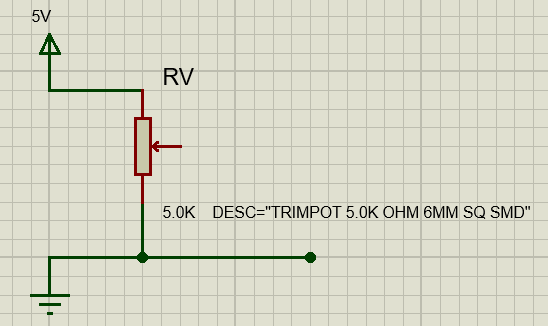
\includegraphics[scale=0.65]{variable_voltage}‎
					\caption{منبع متغیر}
				\end{center}
			\end{figure} 
			
			\item			
			یکی از پایه های تراشه 7400 به منبع متغیر و سر دیگر را همانند شکل مدار زیر به منبع 5 ولت با مقاومت 1 کیلواهم بر سر راه آن وصل میکنیم.
			\begin{figure}[h!]
				\begin{center}
					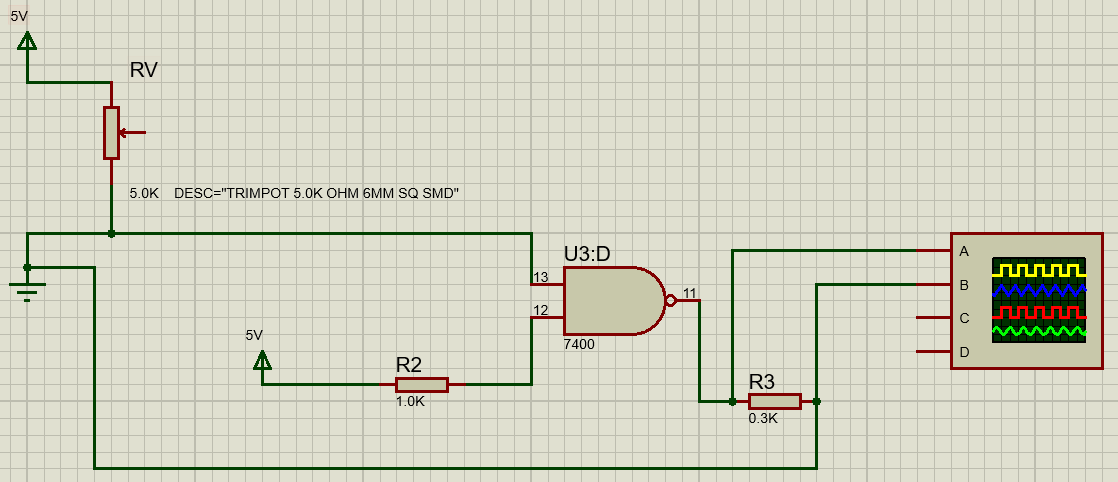
\includegraphics[scale=0.3]{first_madar}‎
					\caption{مدار اندازه گیری مشخصه انتقالی}
				\end{center}
			\end{figure} 
			\item
			برای اندازه گیری ولتاژ خروجی با قرار دادن یک مقاومت 300 اهمی در مدار و اتصال به دو سر اسلیوسکوپ ، جریان و ولتاژ خروجی را اندازه میگیریم. با تغییر دادن مقاومت پتانسیومتر از 0 تا حداکثر مقدار ممکن ولتاژ خروجی منبع متغیر را از 5 تا نزدیکی 0 تغییر میدهیم و با استفاده از مقادیر نشان داده شده توسط اسیلوسکوپ ، نمودار Vi - Vo را رسم میکنیم.
			\item
			حال با تغییر دادن مقاومت پتانسیومتر از مقدار بسیار زیاد حداکثر آن به صفر ، ولتاژ منبع متغیر را از 0 تا 5 تغییر میدهیم و به طور مشابه نمودار Vi - Vo را رسم میکنیم.
			
		\item
		در مرحله بعد آزمایش خروجی گیت NAND را به ورودی های 10 گیت مشابه متصل میکنیم و با تکرار مراحل قبل مجددا نمودار Vi - Vo را رسم میکنیم.
		\begin{figure}[h!]
			\begin{center}
				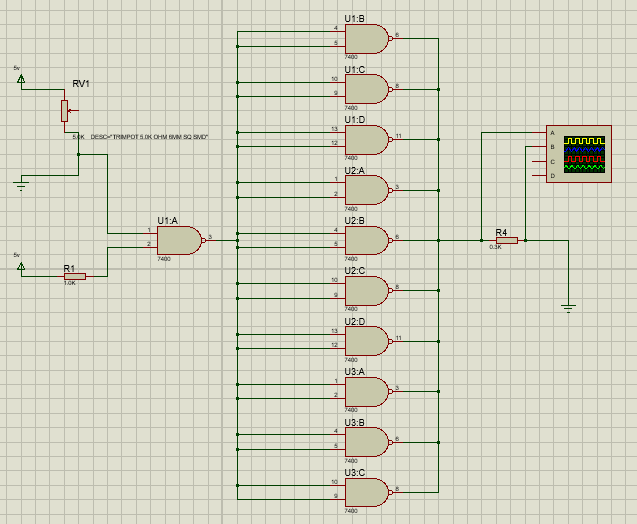
\includegraphics[scale=0.50]{second_madar}‎
				\caption{مدار مرحله آخر آزمایش}
			\end{center}
		\end{figure} 
		\end{itemize}
		
		\newpage
		\subsection*{خلاصه جداول دیتاشیت تراشه های مورد استفاده}
			جداول زیر از این \href{https://cdn.datasheetspdf.com/pdf-down/7/4/0/7400_FairchildSemiconductor.pdf}{منبع} اتخاذ شده اند :
			\begin{figure}[h!]
				\begin{center}
					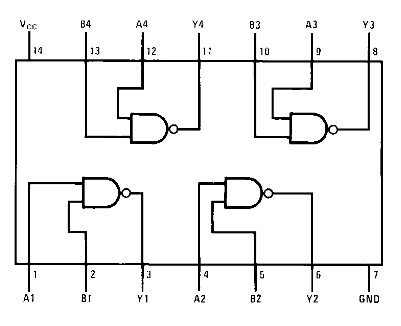
\includegraphics[scale=0.75]{DM74SL00_connection_diagram}‎
					\caption{دیاگرام اتصالات تراشه 7400}
				\end{center}
			\end{figure} 
			\begin{figure}[h!]
				\begin{center}
					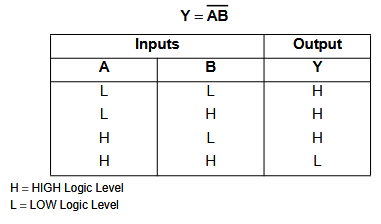
\includegraphics[scale=0.75]{DM74SL00_function_table}‎
					\caption{جدول عملکردی تراشه 7400}
				\end{center}
			\end{figure} 
		
\end{document}









